\cleardoublepage
\chapter{Introduction}
\label{intro}
%\markboth{Introduction}{Introduction}
%\addcontentsline{toc}{chapter}{Introduction}
%A non-numbered chapter\dots

\section{Motivation}
\label{intro_motivation}
% SOURCE: Research plan
The energy sector is currently undergoing big changes in many parts of the world. These changes are driven by two main factors: the need to reduce global CO2 emissions in order to fight climate change, and the opportunities created by digitalisation and the big data era. The share of renewable energies (RE) in the energy mix is growing constantly, with an increasing importance of distributed generation, particularly in urban environments. Rapid improvements in the quantity and quality of data on renewable resources and the environment, as well as in computational methods for data handling and analysis allow to assess the potentials and risks of the developments in the energy sector in unprecedented ways. Focusing on the Swiss energy landscape, this research aims to quantify the potential for distributed hybrid energy generation using state-of-the-art data-driven methods.

More specifically, a spatio-temporal estimation of the potential from two renewable resources in urban environments will be conducted. The potential includes electricity and heat generation from rooftop-mounted solar photovoltaics (PV) and solar thermal collectors, respectively, and heat generation from shallow (<400m) geothermal energy using borehole heat exchangers (BHE). The estimations will be combined with other sources of RE to give a hybrid energy potential that optimally complements the energy demand. While individual aspects have been studied at national scale, no large-scale approach exists to model hybrid potential at high temporal and high spatial resolution to quantify the geographic distribution of storage requirements and maximum energy mismatch. Assessing for the first time the spatio-temporal distribution of hybrid energy potential on national scale can hence give a comprehensive view on the opportunities and risks of hybrid systems and on the regional and national energy balance. 

The first phase of the study focuses primarily on electricity, i.e. the estimation of solar PV potential and its combination with electricity generation from wind and electricity demand (external inputs). During the second phase, heat systems with geothermal and solar thermal heat generation will be investigated. For the computation of potentials, data-driven modelling using Machine Learning algorithms is combined with parallelisation of analytical models to cope with the high spatial and temporal resolution of the relevant datasets. Geographic information systems (GIS) are further used to handle geographically referenced datasets. Efforts are made to quantify the uncertainty related to several modelling steps throughout the study and to identify the sources of uncertainties, for example caused by modelling or by data noise.


\section{A hybrid renewable energy potential for Switzerland}
\label{intro_REN}

Estimation of a hybrid renewable energy potential for Switzerland requires answering the following questions: 
\begin{itemize}
\item Which renewable energy resources are available in Switzerland?
\item How can the potential of these resources be spatially and temporally estimated?
\item What defines a hybrid renewable energy potential?
\end{itemize}

\subsection{Renewable energy in Switzerland}

Two types of renewable energies (RE) will be investigated in this study: solar energy and geothermal energy. These energies are amongst the fastest-growing RE in Switzerland in the last 10 years [1], with growth rates shown in Figure 1. Throughout this study, rooftop-mounted solar installations will be considered for electricity generation from photovoltaic (PV) panels, as well as for heat production for domestic heating and hot water applications from thermal collectors. Geothermal heat generation potential will be calculated for shallow depth (up to 400m) in accordance with current standards for domestic applications. Note that geothermal electricity generation is not considered as this technology is not applied in the domestic sector [2]. 

\begin{figure}[tb] 
\centering 
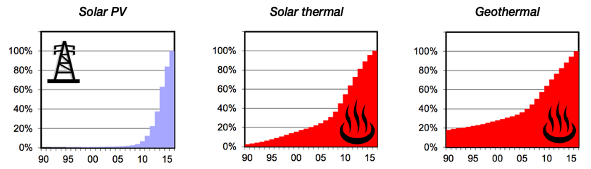
\includegraphics[width=\textwidth]{REN_CH} 
\caption[Growth rates of solar PV, solar thermal and geothermal technology application in Switzerland in the past 25 years.]{Growth rates of solar PV, solar thermal and geothermal technology application in Switzerland in the past 25 years. The data is given in \% of production for 2016 [1].}
\label{fig:ren_ch} 
\end{figure}

\subsubsection{Solar energy from photovoltaics and thermal collectors}

As solar energy is abundantly available and easy to harvest, solar PV and solar thermal technologies have attracted worldwide interest. Most studies of solar potentials focus on PV potentials, for example in Switzerland [3]–[5], USA [6], Spain [7], [8], Germany [9], [10]. Solar thermal potentials on the large scale are rarely quantified; this may be partly due to a lower interest in solar thermal collectors for residential applications [1] and partly due to the high interdependency between collector efficiency and heat demand [11]. Large-scale potential studies have been carried out for thermal power plants in India [12], and for residential buildings in Switzerland [11]. Potentials are typically computed as monthly or yearly values; there is however no current study estimating the large-scale potential at an hourly timescale, which is necessary to quantify a potential for hybrid energy systems and requirements for energy storage. 

\subsubsection{Shallow geothermal energy from borehole heat exchangers}


\subsubsection{Wind energy from large wind turbines}

\subsubsection{Other renewable energy sources}


\subsection{Spatio-temporal estimation of renewable energy potentials}



\subsection{Definition of hybrid renewable energy potential}

\section{Research goals}
\label{intro_goals}
% SOURCE: Research plan
The main driver behind this study is the question whether it is possible to cover urban energy demand in Switzerland using a combination of renewable energies, and which level of energy autonomy could be reached in the built environment from this hybrid renewable energy potential. Special interest lies hereby on the spatial and temporal variability of the supply in order to match the seasonal and intra-day variations of the energy demand. With the focus on two types of resources, solar and geothermal energy, the following research questions arise:

\begin{itemize}
\item How can the potential for renewable energy resources in the built environment be estimated on national scale for Switzerland, and what are the related uncertainties?
\item What impact does the combination of multiple renewable resources to hybrid systems have on distributed energy supply?
\item How can data-driven methods and Machine Learning be applied to improve current ways of estimating potential and to facilitate their scalability to national scale?
\end{itemize}

The above questions have been partly addressed in case studies on building and district scale, or as large-scale studies of individual aspects, but no unified approach exists to assess hybrid energy potential for the built environment at high spatial and temporal resolution. Large-scale potential assessment has been performed in most cases in monthly resolution only, or without considering any spatial distribution of potentials. Many case studies have been conducted, but most models are computationally intensive and infeasible for application the large scale. Furthermore, a comprehensive analysis of uncertainties related to estimation and modelling is rarely provided. Machine Learning has been used in some studies, but there is still a huge potential that can be exploited to understand patterns in the available resources, approximate missing data and model system behaviour in a more computationally efficient way.

This study aims to combine methodologies of large-scale potential assessment and small-scale system modelling to quantify hybrid energy potential in the built environment for Switzerland. Data-driven methods and Machine Learning will be used to overcome gaps caused by lack of data and computational efficiency. The proposed assessment will make use of a large variety of environmental data and will present a unified approach that allows to compare the potential of some of the most promising renewable resources in the built environment. These resources will be combined with the energy demand to derive a hybrid potential which complements the demand patterns. The research hypothesis is hereby that hybrid systems in the built environment bring advantages over single-technology systems, and that a significant fraction of the energy demand can be covered by hybrid renewable potential if the energy mix is chosen appropriately.

The study is divided in three phases. The first phase focuses on electricity. It is divided into the computation of hourly solar energy potentials (WP1) and the assessment of hybrid electricity potential based on solar PV and wind energy (WP2). The second phase focuses on heat energy. In this phase, geothermal energy potentials will be evaluated (WP3) and combined with solar thermal potentials to a hybrid heat potential (WP4). A case study for a selected district will be conducted to assess multi-energy potentials and their effect on covering the urban energy demand. Finally, visualization methods for multi-dimensional data will be explored. 


\section{Structure of the thesis}
To address the above research goals, the thesis is structured as follows:

\textbf{Part~\ref{methods}} provides a summary of state-of-the-art methods used in the thesis and large-scale  datasets used in the national REN potential studies. \textbf{Chapter~\ref{methods_physical}} introduces physical models. \textbf{Chapter~\ref{methods_ML}} covers Machine Learning and uncertainty estimation.  \textbf{Chapter~\ref{data}} provides an overview over the available large-scale datasets.

\textbf{Part~\ref{potential} }addresses the estimation of renewable energy potentials. \textbf{Chapter~\ref{solar} }details the developed model for estimating rooftop solar photovoltaic potential at national scale, as well as a detailed comparison of the resulting potential database with existing estimations for Switzerland. \textbf{Chapter~\ref{geothermal}} provides the estimation of technical potential for shallow geothermal energy, using analytical models at regional scale and Machine Learning for the estimation at national scale. The chapter further shows an approach to expand the model to include thermal regeneration of the geothermal resources through cooling re-injection to the ground with regional-scale application.

\textbf{Part~\ref{hybrid}} shows examples of the application of the potential databases developed in Part~\ref{potential} for case studies on hybrid renewable energy systems. \textbf{Chapter~\ref{hybrid_chapter}} outlines a mapping approach for the energy demand of heat and electricity from readily available data, which is a necessary complementary input to perform hybrid system studies. [TO BE CONTINUED].

\textbf{Chapter~\ref{conclusion}} concludes with the main findings of the thesis and a future outlook.



